

\section{Learning by Gradient Ascent}

\mode<presentation>{
\begin{frame} 
    \begin{center} \huge
        \secname
    \end{center}
    \begin{center}
    i.e. hill climbing
    \end{center}
\end{frame}
}
\notesonly{
Gradient Ascent, i.e. hill climbing
}

\begin{frame}{\secname}
Model parameters can be optimized by stepwise adjustment along the direction of the gradient of the cost function. 

\begin{figure}[h]
  \centering
  \begin{tabular}[c c]{c c}
   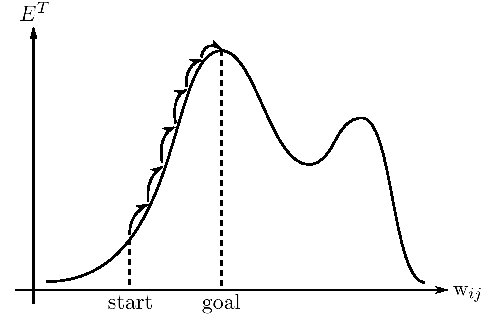
\includegraphics[width=5cm]{img/section2_fig17}
  &\raisebox{2cm}{$\Delta \mathrm{w}_{ij} = \underbrace{ \eta }_{
    \substack{ \text{learning} \\ \text{rate}} }
  \frac{\partial E^T}{\partial \mathrm{w}_{ij}}$}
  \end{tabular}  
  %\caption{Gradient ascent using the training cost}
  \label{fig:gradientDescent}
\end{figure}

\end{frame}

\begin{frame}{\secname}

\slidesonly{
\begin{equation} \label{eq:trainingCost}
	E^T = \ln |\det \vec{W}\,| + \frac{1}{p} \sum\limits_{\alpha = 1}^p
		\sum\limits_{l = 1}^N \ln \widehat{f}_l^{'} \Bigg( 
		\sum\limits_{k = 1}^N \mathrm{w}_{lk} 
		\mathrm{x}_k^{(\alpha)} \Bigg)
\end{equation}

\begin{equation}
\Delta \mathrm{w}_{ij} = 
\eta~\frac{\partial E^T}{\partial \mathrm{w}_{ij}}
 \end{equation}
}

\noindent Taking partial derivatives of the training cost\notesonly{ in \eqref{eq:trainingCost}} w.r.t. the model parameters $w_{ij}$ yields
\begin{equation}
	\frac{\partial E^T}{\partial \mathrm{w}_{ij}}
	= \underbrace{
    \frac{1}{p} \sum\limits_{\alpha = 1}^p 
		\sum\limits_{l = 1}^N \frac{\partial}{\partial \mathrm{w}_{ij}}
		\Bigg\{ \ln \widehat{f}_l^{'} \Bigg( \sum\limits_{k = 1}^N 
		\mathrm{w}_{lk} \mathrm{x}_k^{(\alpha)} \Bigg) \Bigg\}
        }_{ =
			\frac{1}{p} \sum\limits_{\alpha = 1}^p 
			\frac{ \widehat{f}_i^{''} \Big( \sum\limits_{k = 1}^N 
				\mathrm{w}_{ik} \mathrm{x}_k^{(\alpha)} \Big)
			}{\widehat{f}_i^{'} \Big( \sum\limits_{k = 1}^N 
			\mathrm{w}_{ik} \mathrm{x}_k^{(\alpha)} \Big)}
			\cdot \mathrm{x}_j^{(\alpha)} }
		+ \underbrace{ \frac{\partial}{\partial w_{ij}}
			\big( \ln |\det \vec{W}\,| \big) }_{
				\big( \vec{W}^{-1} \big)_{ji} }
\end{equation}

\end{frame}

\begin{frame}{Scope of learning: batch learning}

with an individual cost $e^{(\alpha)}$ for each observation $\vec{x}^{(\alpha)}$:
\begin{equation}
	e^{(\alpha)} = \ln |\det \vec{W}\,| + \sum\limits_{l = 1}^N \ln
		\widehat{f}_l^{'} \Bigg( \sum\limits_{k = 1}^N 
		\mathrm{w}_{lk} \mathrm{x}_k^{(\alpha)} \Bigg)
\end{equation}
The gradient becomes:
\begin{equation}
	\frac{\partial e^{(\alpha)}}{\partial \mathrm{w}_{ij}}
	= \underbrace{ \big( \vec{W}^{-1} \big)_{ji} }_{
		\substack{ \text{costly} \\ \text{computation}} }
		+ \underbrace{  
			\frac{ \widehat{f}_i^{''} \bigg( \sum\limits_{k = 1}^N 
				\mathrm{w}_{ik} \mathrm{x}_k^{(\alpha)} \bigg)
			}{\widehat{f}_i^{'} \bigg( \sum\limits_{k = 1}^N 
			\mathrm{w}_{ik} \mathrm{x}_k^{(\alpha)} \bigg)}
			 }_{ \coloneqq \varphi_i^{(\alpha)} }
		\cdot \mathrm{x}_j^{(\alpha)}
		\label{eq:gradstandardonline}
\end{equation}
this can be used for \emph{batch-learning}:
\begin{equation}
	\Delta \mathrm{w}_{ij}
	= \frac{\eta}{p} \sum\limits_{\alpha = 1}^p 
	\frac{\partial e^{(\alpha)}}{\partial \mathrm{w}_{ij}}
\end{equation}

\end{frame}

\begin{frame}{Scope of learning: online learning}

or using \emph{on-line-learning} by updating $w_{ij}$ with each individual cost $e^{(\alpha)}$ as follows:

\slidesonly{
\begin{algorithm}[H]
  \DontPrintSemicolon
  $t \leftarrow 1$\;
  random initialization of weights $w_{ij}$\;
  \Begin{
    $\eta_t = \frac{\eta_0}{t}$\;
    select next data point $\vec{x}^{(\alpha)}$\;
    change all  $\mathrm{w}_{ij}$ according to:
    $\Delta \mathrm{w}_{ij}^{(t)} = \eta_t \frac{\partial e_t^{(\alpha)}}{\partial
	\mathrm{w}_{ij}} $\;
    $t \leftarrow t + 1$}
%\caption{On-line learning for ICA}
\label{alg:onlineGD}
\end{algorithm}
}
\notesonly{
\begin{algorithm}[h]
  \DontPrintSemicolon
  $t \leftarrow 1$\;
  random initialization of weights $w_{ij}$\;
  \Begin{
    $\eta_t = \frac{\eta_0}{t}$\;
    select next data point $\vec{x}^{(\alpha)}$\;
    change all  $\mathrm{w}_{ij}$ according to:
    $\Delta \mathrm{w}_{ij}^{(t)} = \eta_t \frac{\partial e_t^{(\alpha)}}{\partial
	\mathrm{w}_{ij}} $\;
    $t \leftarrow t + 1$}
%\caption{On-line learning for ICA}
\label{alg:onlineGD}
\end{algorithm}
}

\end{frame}

%\clearpage


\subsection{Natural Gradient Learning}

\subsubsection{Motivation}

\begin{frame}{\subsecname}

\only<1->{
The standard gradient\notesonly{ operates on the notion that }\slidesonly{: }the shortest distance between two points is a straight line.\\ 
}

\notesonly{
A simple counterexample:\\

The shortest distance between two points on a map is not a straight line but rather the shortest ``arc'' connecting those two points on a globe. The natural gradient tries to account for the properties of the surface of the cost function and tries to follow the ``arc'' on that surface.
}

\begin{minipage}{0.45\textwidth}
	\begin{center}
		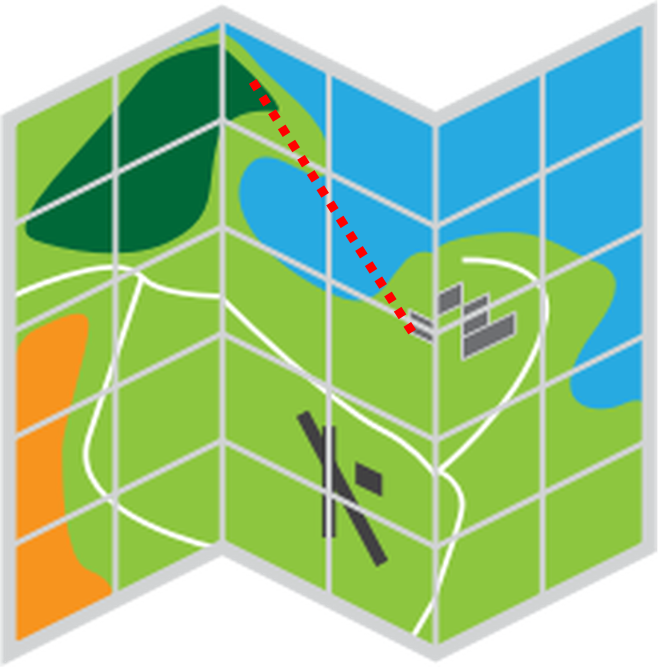
\includegraphics[width=0.7\textwidth]{img/map_icon_markers}  
	\end{center}
	\notesonly{\captionof{figure}{Distances from the viewpoint of the standard gradient.}}
\end{minipage}
\hfill
\begin{minipage}{0.45\textwidth}
	\begin{center}
		\includegraphics<2>[width=0.9\textwidth]{img/globe-icon-2-publicdomain_markers}  
	\end{center}
	\notesonly{\captionof{figure}{Taking the ``arc'' of the surface into account.}}
\end{minipage}

\end{frame}

\subsubsection{Standard gradient vs. natural gradient}

\begin{frame}{\subsubsecname}

\only<1>{
Online learning with standard gradients
\notesonly{requires us to construct a learning rate schedule to ensure we stop overshooting the solution. A decaying learning rate strategy is easier to control if the magnitudes of the gradients are more ``behaved'' you don't suddenly get strong magnitudes that could lead to overshooting the solution. 
}
\slidesonly{
\begin{itemize}
\item can overshoot the solution if we keep a constant learning rate
\item use a decaying learning rate schedule to prevent overshooting
\item a decaying learning rate strategy still sensitive to the magnitude of the gradient,
\end{itemize}
still prone to overshooting.
}
}
\only<2->{
The natural gradient enables \emph{comparable learning steps over time}\footnote{For a more detailed explanation and justification for the natural gradient, see \citep{amari1998natural}}.
It allows for a more stable, therefore efficient, and faster learning rule (no matrix inversion for $\vec W$ in Infomax'
  necessary) to do steepest ascent under normalized step size.%\notesonly{ (cf. lecture slides 2.2.1 for details)}
  
\slidesonly{
\only<2>{
\begin{equation}
	\frac{\partial e^{(\alpha)}}{\partial \mathrm{w}_{ij}}
	= \underbrace{ \big( \vec{W}^{-1} \big)_{ji} }_{
		\substack{ \text{costly} \\ \text{computation}} }
		+ \underbrace{  
			\frac{ \widehat{f}_i^{''} \bigg( \sum\limits_{k = 1}^N 
				\mathrm{w}_{ik} \mathrm{x}_k^{(\alpha)} \bigg)
			}{\widehat{f}_i^{'} \bigg( \sum\limits_{k = 1}^N 
			\mathrm{w}_{ik} \mathrm{x}_k^{(\alpha)} \bigg)}
			 }_{ \coloneqq \varphi_i^{(\alpha)} }
		\cdot \mathrm{x}_j^{(\alpha)}
		%\label{eq:gradstandardonline}
\end{equation}
}
}
  
\begin{equation}
	\Delta \vec{W} = \varepsilon \frac{ \overbrace{\partial e}^{
		\substack{	\text{``original''} \\ 
				\text{gradient}} }}{\partial \vec{W}}
		\underbrace{ \vec{W}^\top \vec{W} }_{
			\substack{	\text{normalization} \\
					\text{of step size}} }
					\label{eq:addnatgradient}
\end{equation}
}

\only<3>{
\notesonly{Applying \eqref{eq:addnatgradient} to the standard gradient in \eqref{eq:gradstandardonline}, }the natural gradient for Infomax becomes:

\begin{equation}
	\Delta \mathrm{w}_{ij} = \varepsilon \sum\limits_{l = 1}^N
	\left\{ \delta_{il} 
	+ \frac{ \widehat{f}_i^{''} \Big( \sum\limits_{k = 1}^N 
			\mathrm{w}_{ik} \mathrm{x}_k^{(\alpha)} \Big)
			}{\widehat{f}_i^{'} \Big( \sum\limits_{k = 1}^N 
			\mathrm{w}_{ik} \mathrm{x}_k^{(\alpha)} \Big)}
	\sum\limits_{k = 1}^N \mathrm{w}_{lk} \mathrm{x}_k^{(\alpha)}
	\right\} \mathrm{w}_{lj}
\end{equation}
}


\slidesonly{
\begin{center}
	\includegraphics<1>[width=0.5\textwidth]{img/section2_fig17}  
\end{center}
}



\end{frame}


% -----------------------------------------------------------------------------
\newpage

\subsection{Choice of transfer function}

\begin{frame}{\subsecname}
%\subsection{Choice of $\widehat{f}_i$:}
The true distribution is typically unknown, 
but likely to have a probability density with one maximum (i.e. peaky function)
$\leadsto$ cdf of this unknown source distribution will be roughly sigmoidal.\\

A typical choice to resemble the cdf of such a peaky function:

\slidesonly{
\begin{center}
	\includegraphics<1>[width=0.7\textwidth]{img/section2_fig15}  
\end{center}
}
\only<2>{

\svspace{-10mm}

\begin{equation} \tag{logistic function}
	\widehat{f}_{(y)} = \frac{1}{1 + \exp(-y)}
\end{equation}
\begin{equation}
	\frac{\widehat{f}_{(y)}^{''}}{\widehat{f}_{(y)}^{'}}
	= 1 - 2 \widehat{f}_{(y)}
\end{equation}
Observation: ICA is fairly robust against false choice of $\widehat{f}$.

\begin{itemize}
	\itR however: if $\widehat{f}_i$ deviates too strongly from its true
		shape, the fixed point may become unstable
	\itR if in doubt (and enough training data is available)
	\begin{itemize}
		\itl make a parametrized ansatz for $\widehat{f}_i$
		\itl estimate parameters in addition to $\vec{W}$
	\end{itemize}
\end{itemize}
}

\end{frame}
